\documentclass[tikz]{standalone}
\usetikzlibrary{intersections}

\begin{document}
	\begin{tikzpicture}[line width = 0.3mm]
	
	\node[anchor = north west, inner sep = 0, outer sep = 0] (I) at (0, 0) 
					{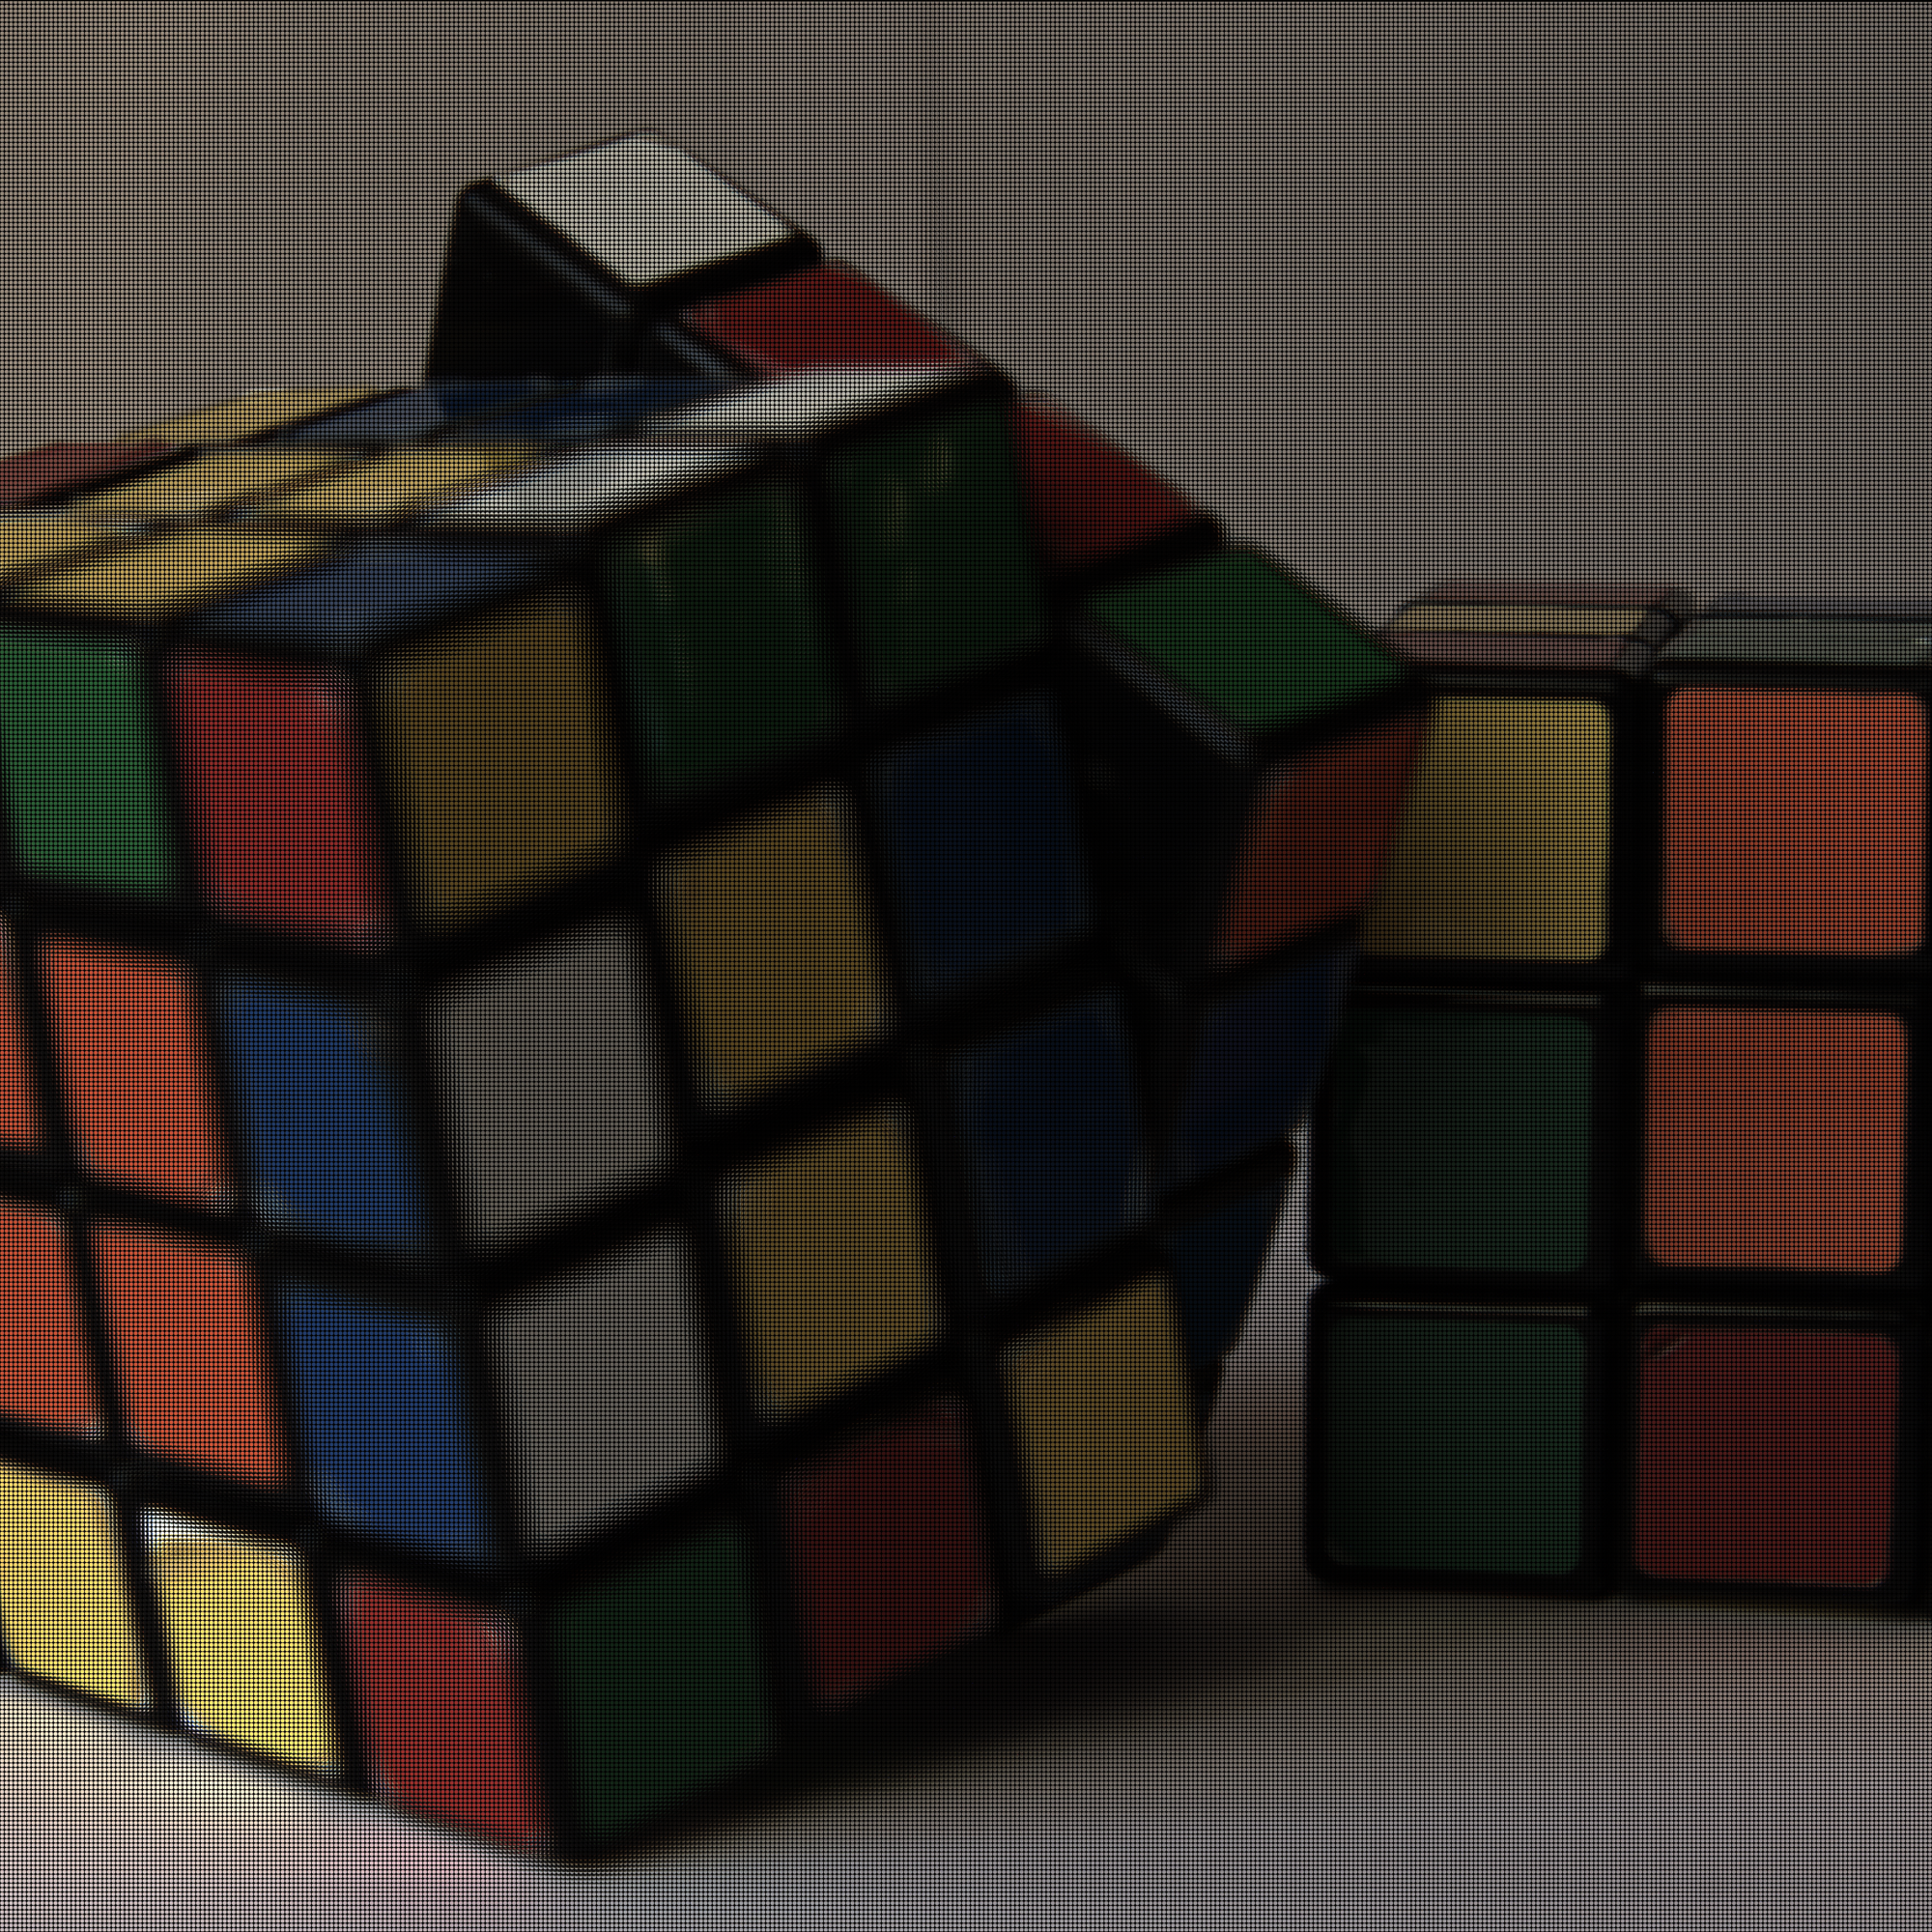
\includegraphics[width = 5.5cm]{../Figures/lytro/lenslet_view_2000.png}};
	% full size = 7378, cropped size = 500
	% zoom box anchor at (955, 2200) in full image matrix
	\coordinate (A) at (955 * 5.5 / 7378, -2200* 5.5 / 7378);
	\coordinate (S) at (500 * 5.5 / 7378, -500 * 5.5 / 7378);	
	\draw[blue, line width = 0.5mm] (A) rectangle ++(S); 
	
	% Magnification box
	\node[anchor = north west, xshift = 0.3cm, inner sep = 0pt] (I2) at (I.north east) 
					{\includegraphics[width = 5.5cm]{../Figures/lytro/lenslet_array_zoom_at_955_2200_500x500.png}};
	\begin{scope}
		\clip (I2.south east) rectangle (I2.north west);
		\draw[blue, line width = 2.5mm] (I2.south east) rectangle (I2.north west);
	\end{scope}
	
	
	
	\end{tikzpicture}
\end{document}
